
\section{Background and Preliminaries}
\label{sec:background}
We start with some background on key technical concepts and notation needed for the rest of this paper.
\subsection{Deep Learning}
Deep learning (DL) refers to a technique for approximating patterns within data by applying gradient descent to optimize the parameters of a directed graph of operators. In this paper, we refer to the DL model graph as a \textit{model}, or a \textit{neural computational graph}. Feedforward networks are a particular type of computational graph wherein inputs are continuously fed forward through a chain of operators, each of which is known as a layer. Most large-scale model architectures fall under this class.

Common DL operators include \textit{matrix multiplies}, \textit{differentiable activation functions}, and \textit{embedding table lookups} (functionally equivalent to matrix multiplies with one-hot vectors). The first two are used for directly transforming data inputs while the latter is used for associating some personalized vector with a categorical input (e.g. translating an application user into a vector). A DL model might use all of these operators together in a complex structure, typically known as a deep neural network (DNN).

The \textit{training} of a model involves an optimization procedure called stochastic gradient descent (SGD). It samples \textit{mini-batches} of data from the training dataset, then runs a \textit{forward} pass through the model graph. The forward pass transforms the input data features into an output target, then calculates a \textit{loss} value, or error, relative to some ground truth \textit{label}. This loss value is used to run a \textit{backward} pass, also known as backpropagation. Backpropagation refers to the process of repeatedly applying the chain rule to calculate updates for each model parameter that will minimize the output loss. Note that in order for this chain process to work, intermediate outputs, also known as \textit{activations}, between operators \textit{must be saved}. \textit{Inference} applications, wherein the model parameters is frozen deployed for prediction, can discard intermediate outputs when transforming inputs, but training has to save the intermediates (which can bloat memory costs).

A full pass of minibatch samples through the entire dataset is called an \textit{epoch}. Training a model typically requires many epochs of SGD. Popular DL tools implement many variants of SGD (e.g., Adam, AdaGrad, RMSProp, etc.), known as \textit{optimizers} but their data access patterns are identical. Some optimizers maintain their own parameters and state which are updated during execution.

The size of a DL model can be measured through the number of parameters and/or its memory footprint. The memory footprint of a model is generally correlated with the number of parameters. In order to compute a full minibatch-pass, intermediate data must be materialized between layers, and gradients will also need to be held in memory as they are chained backwards during backpropagation. As such, an upper bound of model memory footprint can be made based on the sum of its parameters' memory costs, its intermediates' memory costs, and its gradients' memory costs. This upper bound is generally a high overestimate, since most training frameworks will automatically discard intermediates and gradients as soon as they are no longer needed.

\subsection{Deep Learning Accelerators}
Matrix multiplies are typically the most common and computationally intensive operators within DL model graphs. Other operators exist (e.g. activation functions, embedding table lookups) but these are generally less computationally intense. The general matrix multiply operation, or GEMM, is a well studied target for parallelization~\cite{blislab2016}. As such, using hardware that can exploit this opportunity effectively is a common practice among DL model developers.

\textbf{GPUs} offer stronger parallelization capabilities versus CPUs for simple operations such as the GEMM. In particular, Nvidia GPUs support the cuDNN library~\cite{cudnn}, which implements low-level DL operators tuned for parallelization on GPU threads. However, GPUs must operate on data stored within on-accelerator memory, which is far more limited than standard system memory (DRAM). A state-of-the-art consumer GPU typically has less than 40GB of on-device memory, while DRAM capacity on a training machine might easily exceed 512GB. 

\textbf{TPUs}, or tensor processing units, are a new type of accelerator developed by Google specifically for DL. TPU cores are organized to support parallelism in GEMM operations and experimental evaluations show that it can achieve up to 10X faster performance than GPUs on some model architectures~\cite{tpubenchmark2019}. Unfortunately, TPU access is still very limited --- practitioners can only use one through Google's Cloud Platform. As such, this survey will primarily focus on systems targeting GPU execution.

\subsection{Parallelization Techniques}\label{sec:parallelization}
A variety of techniques exist for parallelizing DL training. Each offers different advantages or drawbacks, which tend to vary depending on the workload. Understanding the data access and communication patterns of each strategy is critical to evaluating them in the context of large-model training.

\textbf{Model parallelism} refers to the technique of partitioning, or \textit{sharding}, a neural architecture graph into subgraphs known, and assigning each subgraph, or \textit{model shard} to a different device. In a feedforward network, these shards might refer to groups of stacked layers.

\begin{figure}[th!]
\centering
	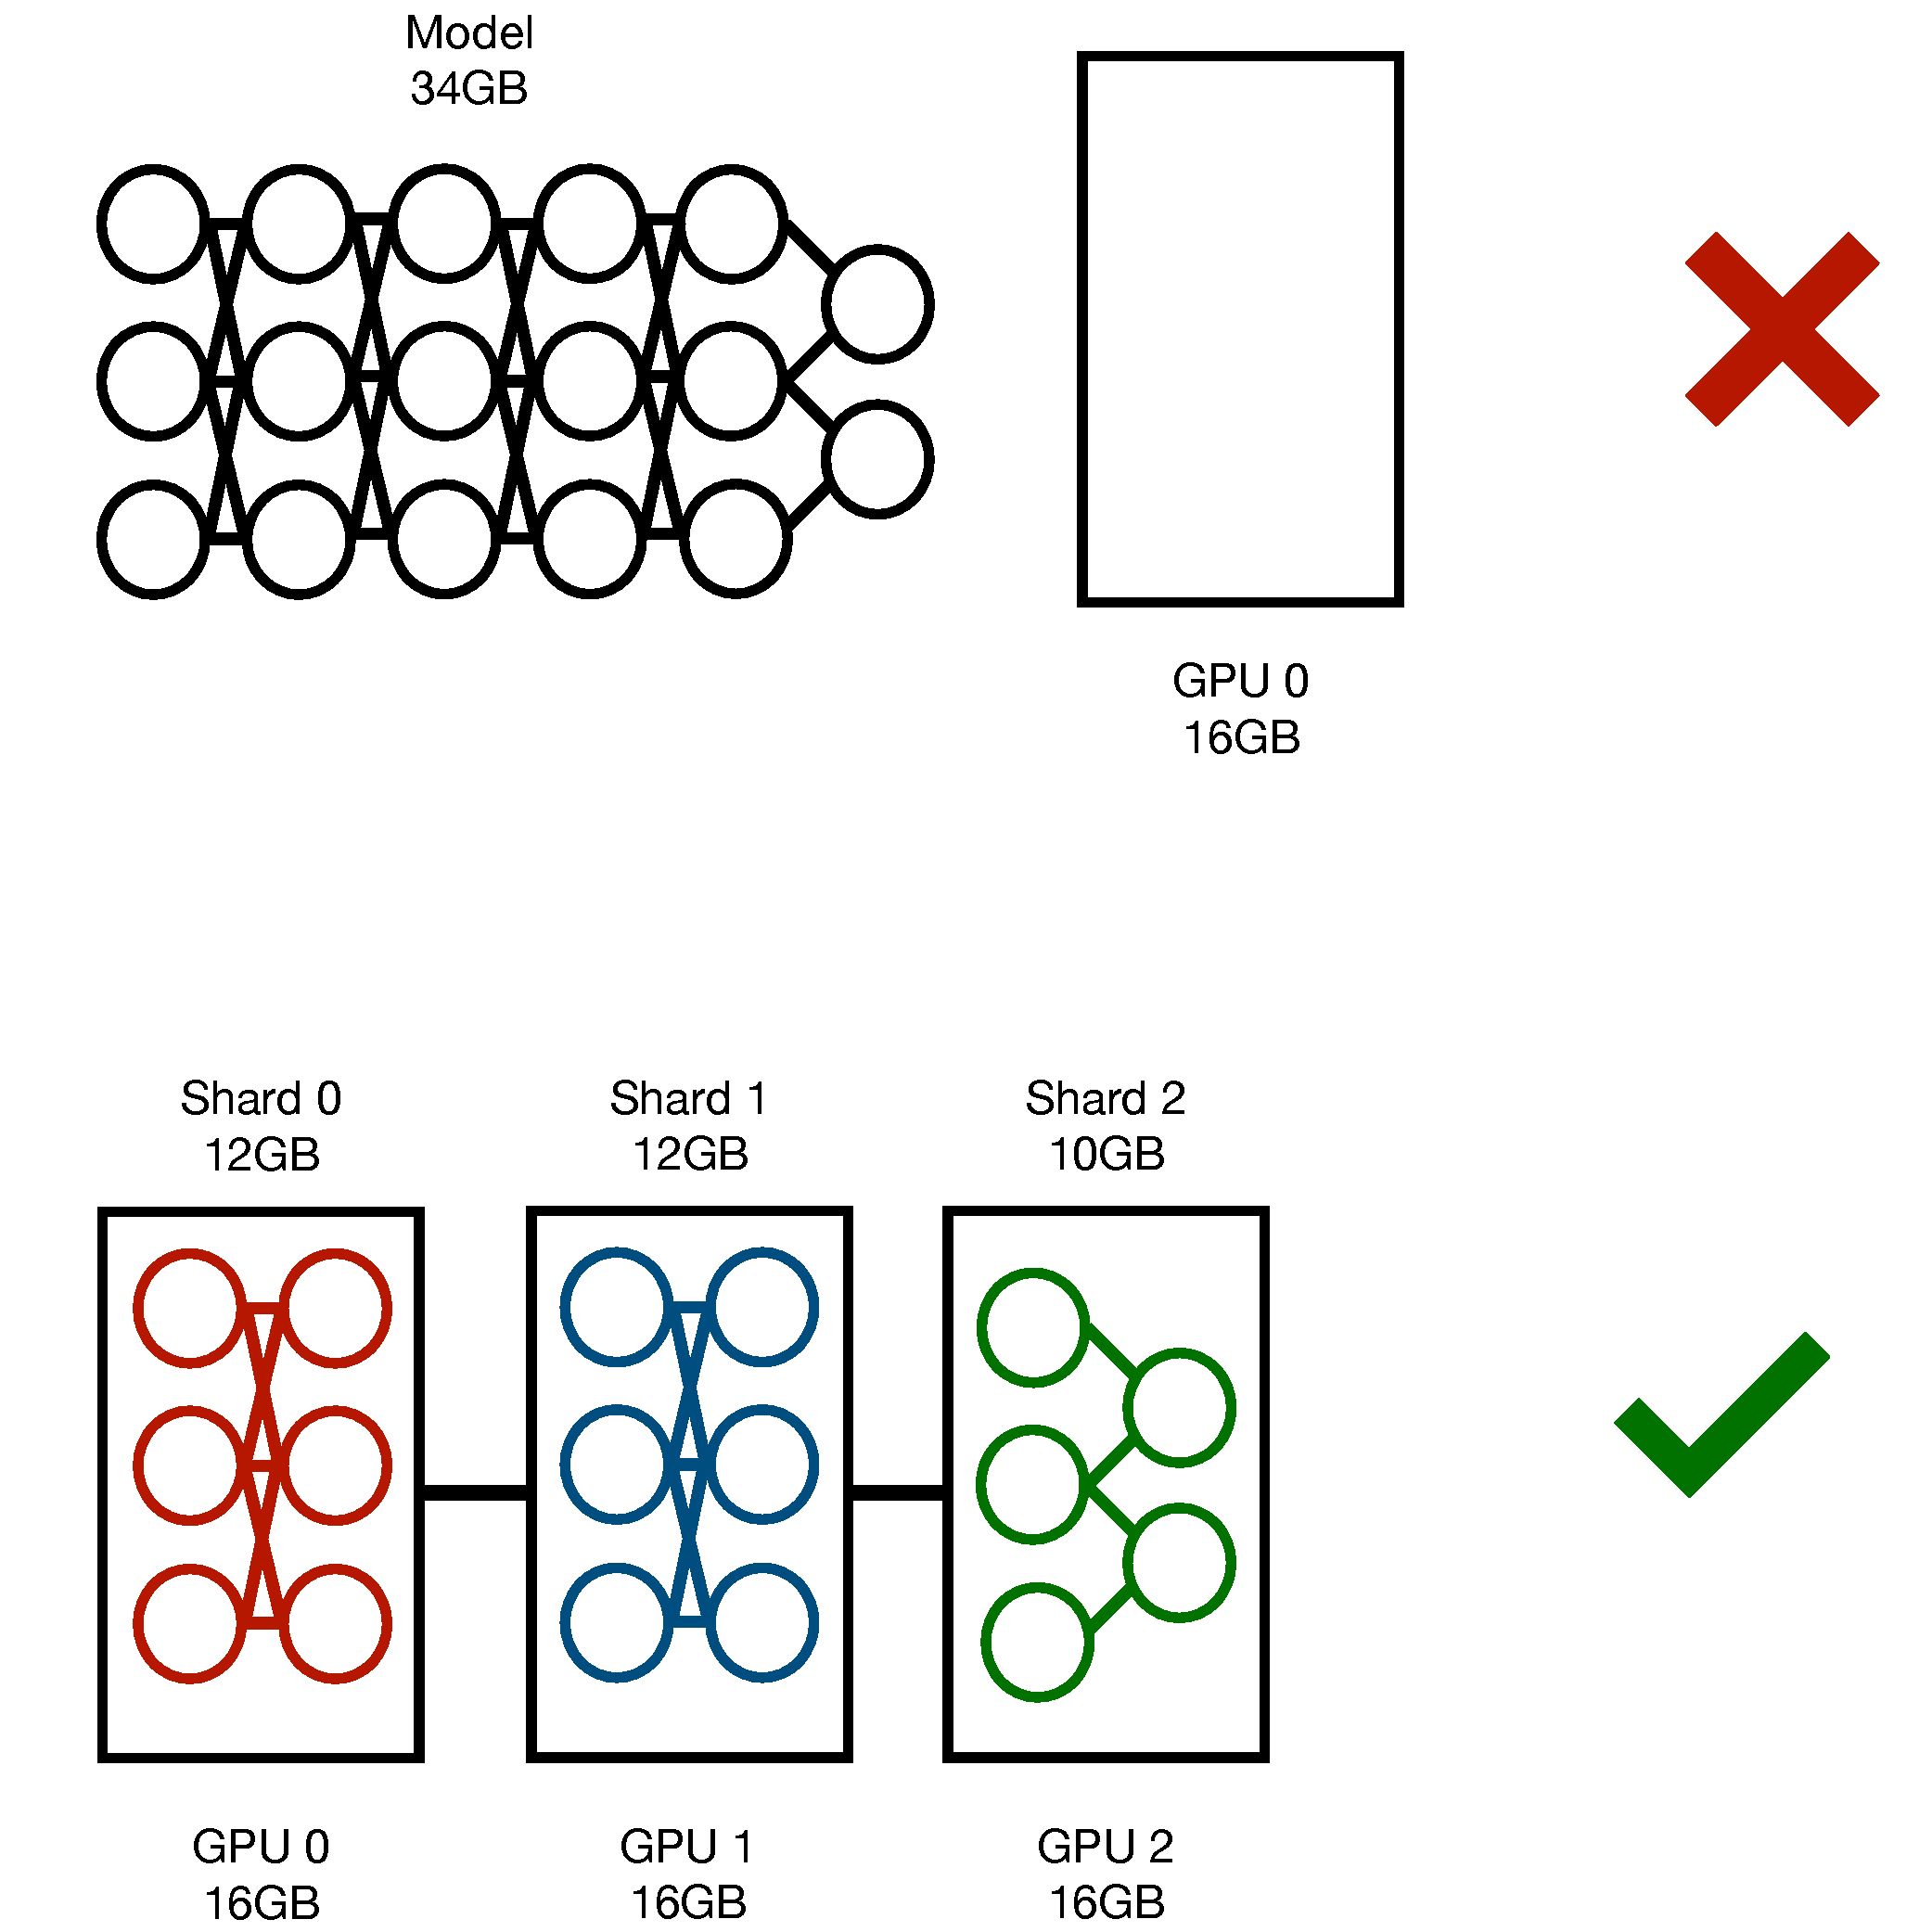
\includegraphics[keepaspectratio=true, width=0.9\linewidth]{images/model_parallelism_basic}
	\caption{An illustration of how a large feedforward network that does not fit into a single GPU could be model-parallelized over three GPUs to enable execution. Note that execution has not been sped up --- there is no parallel execution, only partitioned memory demands.}
	\label{fig:model_parallel_feedforward}
\end{figure}


The speedup potential of model parallelism depends largely on the architecture and the sharding strategy. Sequential model parallelism on a feedforward network, of the sort illustrated in Figure~\ref{fig:model_parallel_feedforward} will offer no scope for parallel execution, instead inducing a dependency graph between accelerators. This sharding strategy is still popular, however, as it can distribute memory demands across multiple devices and is fairly simple to setup. Other operators, such as embedding tables, are more amenable to being sharded width-wise as illustrated in Figure~\ref{fig:embedding_table_parallel}. Width-wise sharding strategies, more generally known as \textit{tensor parallelism}, can execute layers in parallel across multiple devices, but typically need to be followed by an all-gather communication pattern to produce a full output.

\begin{figure*}[th!]
\centering
	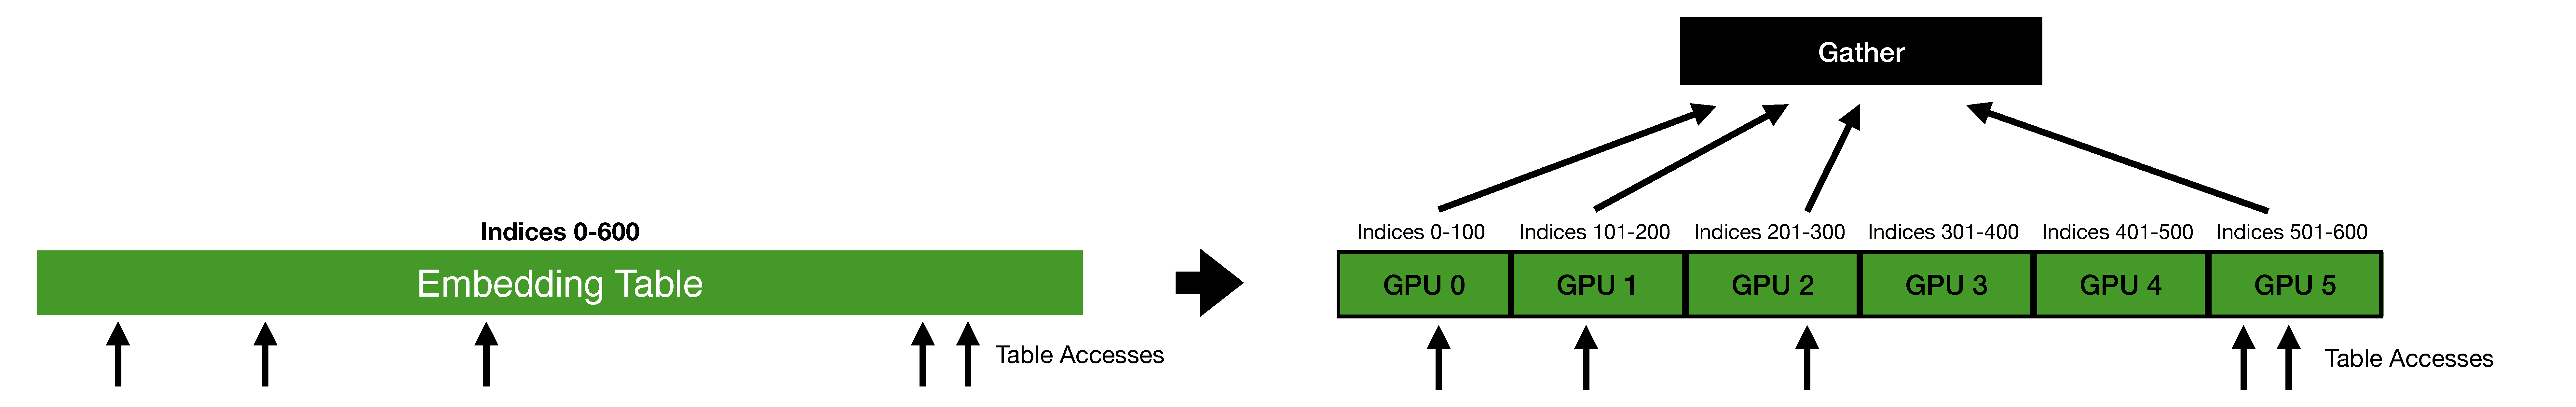
\includegraphics[keepaspectratio=true, width=0.9\linewidth]{images/embedding_table_parallel}
	\caption{An embedding table parallelized over 6 GPUs. Each GPU receives a different subset of the table's indices.}
	\label{fig:embedding_table_parallel}
\end{figure*}

Model parallelism of any sort introduces GPU-GPU communication. The latest Nvidia GPUs support ``NVLink'' interconnects --- high-speed GPU-GPU communication routes that offer as much as 900GB/s bandwidth --- which can help minimize overheads. NVLink is not always readily available, however, particularly when using cloud-provided machines that the user cannot customize easily. When NVLink is not supported, GPU-GPU communication runs over PCiE interconnects, which are much slower. The Tesla V100, generally considered a standard high-performance GPU for DL applications, supports a 16-lane PCiE 3.0 interconnect, at 16GB/s. 

To avoid having to transfer too much data over slow interconnects, model parallelism users generally aim to select a partitioning strategy that will minimize the size of activations that need to be transferred between shards, or else balance out computation to hide communication costs. Various sharding algorithms exist for this~\cite{flexflow2018,gpipe2019,lamp2020,mpanalysis2019,hydra2021,zero2019}.

\textbf{Data parallelism} is a common deep learning execution strategy that enables multiple mini-batches of data to be consumed in parallel. Data parallel execution techniques can be divided into two broad categories --- asynchronous data parallelism and synchronous data parallelism. 

The most well-known asynchronous technique is Parameter Server, wherein one core chief server holds a baseline set of parameters while distributed workers hold model replicas that train on different minibatches. The distributed workers occasionally send updates to the baseline server, which in turn will send out replacement parameters to the distributed workers to keep them updated. The workers can run out of sync with each other, as they only need to communicate/synchronize with the baseline server. Asynchronous techniques introduce many challenges, such as accuracy degradation versus single-worker training and irreproducible results due to variance in worker return times. For these reasons, asynchronous techniques are relatively uncommon in the modern DL training landscape. 

The most popular synchronous data parallel execution technique is Distributed Data Parallelism (DDP). DDP replicates a model and assigns copies to $m$ different accelerators. These replicas consume different minibatches of size $n$ in parallel and produce gradient updates for their local replica. These gradients are then aggregated across replicas to produce a global update, typically using an all-reduce communication pattern. This global update is then applied to every replica in parallel. This technique is mathematically equivalent to single GPU training with batch size $m \times n$. While this technique induces an all-reduce communication step, these overheads can generally be overlapped and hidden under model execution times.

\textbf{Hybrid parallelism} refers to strategies which \textit{combine} different parallelization strategies to achieve higher overall performance. For example, overlaying data parallelism on top of model parallelism could enable a user to achieve memory scalability across multiple devices along with the execution speedups of data parallelism. These strategies have tradeoffs that need to be factored into their design. In a simple overlay hybridization, model parallelism's multi-device requirements are multiplied by the replication requirements of data parallelism. A further overlay of task parallelism (e.g. in multi-model training) could add another multiplication factor into the equation. More complex hybridizations are covered in Section~\ref{sec:mlsys}.

\subsection{Model Modification}
Another approach is to actually reduce or alter the model itself to reduce its memory demands. Various techniques for \textit{compression} exist, some dynamic that readjust the architecture during training, and other static ones that reduce the model up front. Typically, compression induces an accuracy-size tradeoff, where higher compression factors reduce model learning capacity. This tradeoff can make this technique ill-suited to accuracy-critical applications, though well-managed and strategic compression can minimize the accuracy loss.

\textbf{Model distillation} attempts 

















